\chapter{Аналитический раздел} 

\section{Анализ предметной области}
Компьютерный магазин предлагает разнообразный ассортимент продукции, включая компьютеры, комплектующие, периферийные устройства, программное обеспечение и аксессуары. Для эффективного управления ассортиментом необходимо учитывать такие характеристики товаров, как название, описание, производитель, цена, количество на складе и уникальный идентификатор товара. \cite{2}

Одной из ключевых задач является поддержание актуальной информации о количестве товаров на складе. 

Система должна поддерживать функции создания, редактирования и отслеживания заказов. Это включает информацию о клиентах, деталях заказа (список товаров, количество, стоимость) и статусах заказов (оформлен, обработан, доставлен и т.д.). Кроме того, важно отслеживать статусы заказов, такие как "оформлен"  \,, "обработан"  \,, "в пути" и "доставлен" \ чтобы обеспечить своевременную и точную обработку каждого заказа. \cite{3}

Для повышения качества обслуживания необходимо вести учет данных о клиентах, таких как имя, контактная информация, история покупок. Это поможет персонализировать предложения и улучшить клиентский сервис. \cite{3}
\newpage
\section{Постановка задачи}
Разработка удобного программного обеспечения для управления данными компьютерного магазина. Пользователи могут просматривать товары, размещать заказы и отслеживать информацию о заказе, а владельцы магазинов — управлять данными о товарах и заказах.

На рисунке \ref{img:idef0} приведена IDEF0-схема для поставленной задачи.
\begin{figure}[ht!]
	\centering
	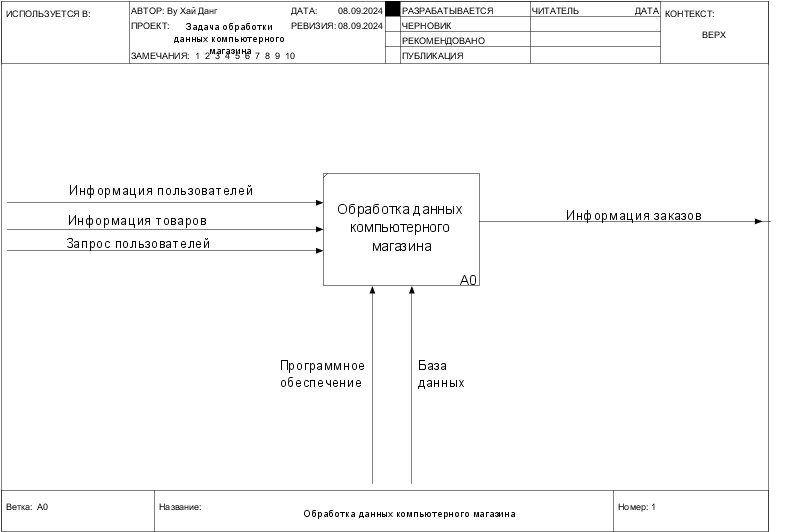
\includegraphics[width=1\linewidth]{img/1.jpg}
	\caption{Функциональная модель поставленной задачи}
	\label{img:idef0}
\end{figure}

\newpage
\section{Формализация данных}

В базе данных хранится информация о:
\begin{itemize}[label=---]
	\item пользователях;
	\item товарах;
	\item заказах;
	\item корзинах
	\item деталях корзины
	\item деталях заказы
	\item промокодах
\end{itemize}

В таблице \ref{table:anal1} приведены информации о каждой сущности.
\begin{table}[ht!]
	\caption{Категории и сведения о данных}
	\label{table:anal1}
	\begin{center}
		\begin{tabular}{|c|p{9cm}|}
			\hline
			\textbf{Категория} & \textbf{Сведения}\\
			\hline
			Пользователь & Имя, номер телефона, адрес, почта, логин, пароль, права доступа.\\
			\hline
			Товар & Название, цена, количество, производитель, описание.\\
			\hline
			Промокод & Код, акция, дата начала, дата конца.\\
			\hline
			Корзина & Дата создания, Пользователя.\\
			\hline
			Деталь корзины & Товары, корзины, количество.\\
			\hline
			Заказ & Пользователя, промокода, статус, дата создания. \\ 
			\hline
			Деталь заказа & Пользователя, заказа, количество.\\
			\hline
		\end{tabular}
	\end{center}
\end{table}

\newpage

На рисунке \ref{img:er-dia} отображена ER-диаграмма системы, основанная на приведенной выше таблице.
\begin{figure}[ht!]
	\centering
	\includegraphics[width=0.8\linewidth]{img/ER_dia.png}
	\caption{ER-диаграмма}
	\label{img:er-dia}
\end{figure}
\newpage
\section{Системные пользователи}

Для взаимодействия с программным обеспечением было выделено четыре вида ролей пользователей: гость, администратор, поставщик и клиент. Каждая из ролей обладает различными правами доступа и функциональностью, адаптированной к их задачам.

\begin{enumerate}
	\item Гость: имеет право только регистрировать информацию;
	\item Администратор: обладает максимальными правами доступа. В его компетенции управление всем приложением, включая редактирование и удаление товаров, управление пользователями, редактирование заказов;
	\item Поставщик: ответственен за добавление новых товаров и управление их количеством на складе. Он может обновлять информацию о продуктах, включая цены, описания и наличие на складе;
	\item Клиент: имеет возможность оформлять заказы, просматривать свою историю покупок, редактировать личные данные. Клиенты могут взаимодействовать с корзиной товаров и отслеживать статус своих заказов.
\end{enumerate}


На рисунке \ref{img:user-case} представлена Use-Case диаграмма пользователей.
\begin{figure}[ht!]
	\centering
	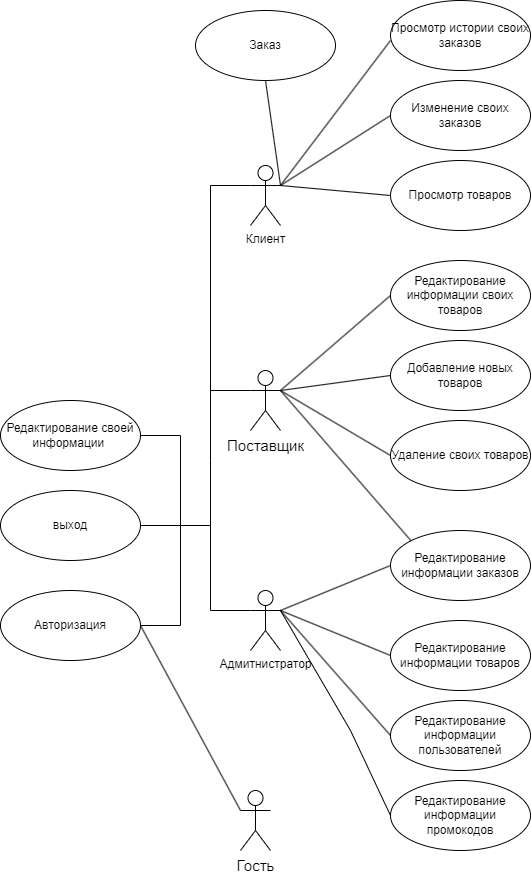
\includegraphics[width=0.5\linewidth]{img/user_case.png}
	\caption{Use-Case диаграмма}
	\label{img:user-case}
\end{figure}

\newpage
\section{Модель баз данных}
\textbf{Модель данных} --- это совокупность допустимых структур данных и операций над ними, поддерживаемая компьютерной средой (в т. ч. СУБД), для определения логической структуры базы 
данных и динамического моделирования состояний предметной области. \cite{bd-1}

Модели данных действительно  разделятся на три основных вида: дореляционные, реляционные и постреляционные. Каждый из этих видов моделей данных характеризуется своими особенностями, архитектурой и областями применения.

\subsection{Дореляционные модели данных}
Иерархическая база данных организована в виде множества деревьев, где каждый узел дерева представляет собой запись, содержащую именованные поля, соответствующие атрибутам объектов предметной области. В такой структуре данные упорядочены по строгой иерархии: каждая запись-«потомок» может иметь только одну запись-«родителя», исключая возможность наличия нескольких предков. Этот подход используется для представления отношений, когда данные имеют четкую и логичную иерархическую структуру. \cite{csharp}

Одним из основных ограничений иерархических баз данных является трудность представления более сложных взаимосвязей, таких как отношения «многие-ко-многим». В такой структуре данные жёстко связаны, что усложняет внесение изменений или расширение системы, особенно если данные не вписываются в строгую иерархию. Также требуется дублирование данных, если одни и те же «потомки» должны быть связаны с несколькими «родителями», что приводит к избыточности.

На рисунке \ref{img:1_model} представлена иерархическая модель данных в базе данных интернет--провайдера.
\begin{figure}[ht!]
	\centering
	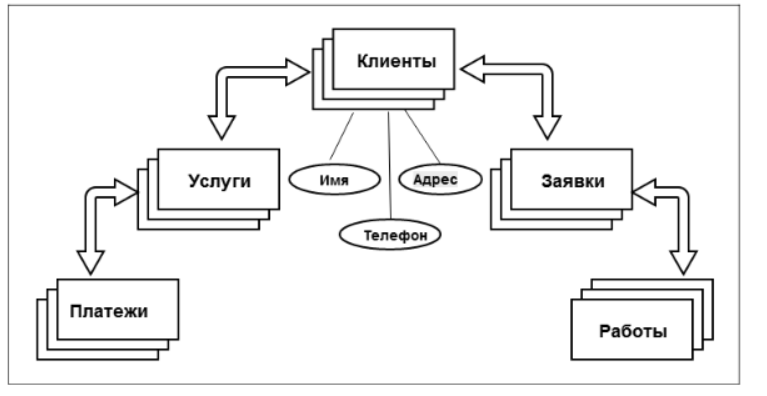
\includegraphics[width=0.55\linewidth]{img/2.png}
	\caption{Фрагмент иерархической модели данных}
	\label{img:1_model}
\end{figure}

Сетевая модель данных организована в виде графа, где записи представляют собой узлы, соединенные между собой множественными отношениями. В отличие от иерархической модели, узел в сетевой базе данных может иметь несколько родительских и несколько дочерних узлов, что позволяет более гибко моделировать сложные взаимосвязи между данными. Эта структура особенно полезна для представления и управления данными, которые не вписываются в жесткую иерархическую структуру, позволяя создавать более сложные и разветвленные сети взаимосвязей. \cite{csharp}

Одним из ключевых преимуществ сетевой модели является её высокая производительность при выполнении сложных запросов, так как она позволяет напрямую переходить между связанными узлами без необходимости прохода через промежуточные уровни, как это происходит в иерархической модели. Это делает её эффективной для обработки больших объемов данных с множеством взаимосвязей.

На рисунке \ref{img:2_model} представлен фрагмент сетевой модели данных в базе данных интернет--провайдера.
\begin{figure}[ht!]
	\centering
	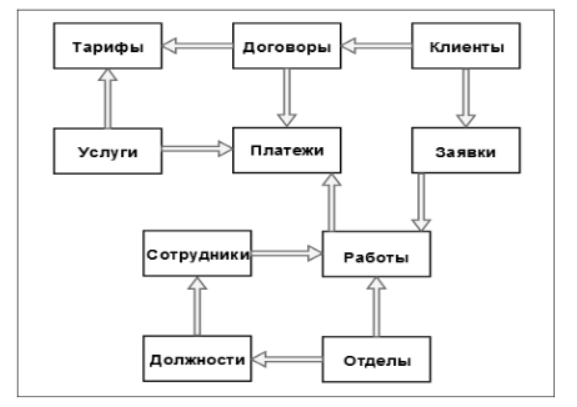
\includegraphics[width=0.55\linewidth]{img/3.png}
	\caption{Фрагмент иерархической модели данных}
	\label{img:2_model}
\end{figure}

\subsection{Реляционные модели данных}

Реляционная база данных представляет собой набор взаимосвязанных таблиц, каждая из которых имеет уникальное имя. Таблицы отображают данные о реальных объектах или «сущностях» предметной области и состоят из строк, называемых кортежами, и столбцов, называемых атрибутами. Каждый кортеж представляет собой экземпляр сущности и описывается набором значений, соответствующих его атрибутам. Для установления связей между таблицами используется механизм внешних ключей: эти ключи содержат ссылки на соответствующие атрибуты других таблиц, обеспечивая целостность данных и возможность выполнения сложных запросов. \cite{csharp}

Одной из ключевых особенностей реляционных баз данных является возможность их масштабирования и высокой совместимости с различными приложениями и системами. В то же время, для сложных структур данных, таких как графы или документы, реляционная модель может быть менее эффективной, так как требует преобразования таких данных в таблицы, что иногда приводит к усложнению запросов и снижению производительности.

На рисунке \ref{img:3_model} представлен пример реляционной модели данных
\begin{figure}[ht!]
	\centering
	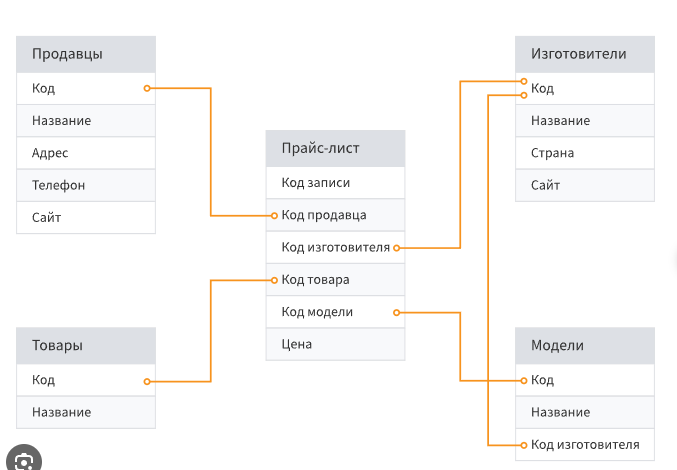
\includegraphics[width=0.55\linewidth]{img/4.png}
	\caption{Пример реляционных моделей данных}
	\label{img:3_model}
\end{figure}

\subsection{Постреляционные модели данных}
Современные постреляционные СУБД обладают гибкостью, позволяющей хранить и обрабатывать разнообразные типы данных, включая документы, графы и мультимедийные объекты. Это делает их особенно полезными для приложений, требующих работы с большими объемами неструктурированных данных, таких как социальные сети, системы рекомендаций и аналитика больших данных. Важной особенностью постреляционных СУБД является поддержка расширяемых схем данных, что позволяет динамически изменять структуру базы данных без значительных затрат на её перестройку.

\subsection{Выбор модели данных}

Реляционная модель данных была выбрана из-за её зрелости и надежности, что делает её стандартом для многих критически важных приложений. Она обеспечивает строгую целостность данных через механизмы ограничений и поддержку транзакций, что помогает избежать несоответствий и потери данных. Кроме того, реляционная модель позволяет обеспечить независимость данных от приложения, что упрощает модификацию структуры данных и делает систему более адаптируемой к изменяющимся требованиям бизнеса. \cite{god}

\subsection*{Вывод}

В данном разделе была проведена формализация задачи и данных, рассмотрены типы пользователей и требуемые функционалы. Также был проведен анализ существующих моделей баз данных и было решено использовать в данной работе реляционную СУБД.

